\documentclass{report}

\usepackage{amsmath, amsthm, amssymb, amsfonts}
\usepackage{thmtools}
\usepackage{graphicx}
\usepackage{subcaption}
\usepackage{setspace}
\usepackage{geometry}
\usepackage{float}
\usepackage{hyperref}
\usepackage[utf8]{inputenc}
\usepackage[english]{babel}
\usepackage{framed}
\usepackage[dvipsnames]{xcolor}
\usepackage{tcolorbox}
\usepackage{multicol}
\usepackage{minted}

\colorlet{LightGray}{White!90!Periwinkle}
\colorlet{LightOrange}{Orange!15}
\colorlet{LightGreen}{Green!15}

\newcommand{\HRule}[1]{\rule{\linewidth}{#1}}

\declaretheoremstyle[name=Theorem,]{thmsty}
\declaretheorem[style=thmsty,numberwithin=section]{theorem}
\tcolorboxenvironment{theorem}{colback=LightGray}

\declaretheoremstyle[name=Proposition,]{prosty}
\declaretheorem[style=prosty,numberlike=theorem]{proposition}
\tcolorboxenvironment{proposition}{colback=LightOrange}

\declaretheoremstyle[name=Principle,]{prcpsty}
\declaretheorem[style=prcpsty,numberlike=theorem]{principle}
\tcolorboxenvironment{principle}{colback=LightGreen}

\setstretch{1.2}
\geometry{
    textheight=9in,
    textwidth=5.5in,
    top=1in,
    headheight=12pt,
    headsep=25pt,
    footskip=30pt
}

% ------------------------------------------------------------------------------
\tcbset{
    sharp corners,
    colback = white,
    before skip = 0.2cm,    % add extra space before the box
    after skip = 0.5cm      % add extra space after the box
}                           % setting global options for tcolorbox

\definecolor{main}{HTML}{5989cf}    % setting main color to be used
\definecolor{sub}{HTML}{cde4ff}     % setting sub color to be used

\newtcolorbox{boxH}{
    colback = sub, 
    colframe = main, 
    boxrule = 0pt, 
    leftrule = 6pt % left rule weight
}

\newcommand{\SubItem}[1]{
    {\setlength\itemindent{15pt} \item[-] #1}
}

% ------------------------------------------------------------------------------

\begin{document}

% ------------------------------------------------------------------------------
% Cover Page and ToC
% ------------------------------------------------------------------------------

\title{ \normalsize \textsc{}
		\\ [2.0cm]
		\HRule{1.5pt} \\
    \LARGE \textbf{\uppercase{Computer forensics and Cyber crime analysis}}
		\HRule{2.0pt} \\ [0.6cm] \LARGE{Thats a lot of words in the title} \vspace*{10\baselineskip}}
\date{}
\author{\textbf{Fabio Lorenzato}} 
		

\maketitle
\newpage

\tableofcontents
\newpage

% ------------------------------------------------------------------------------

\part{Legal part}
\chapter{Introduction}
Back in the days, it was really easy to analyze the communication between two people, because the
technology was easier and know, meaning that the technology is \textit{between us}. Nowadays the
technology is more \textit{about us}, for example we use AI for facial recognition. Another example
are the social network algorithms that track our activity online. This means that we use the
technology to be "analyzed" instead of using it only to communicate. Most likely, the technology
will be \textit{in us}, which not only means robotics, but also be more integrated with human
beings.\\
In those scenarios, computer forensics became more complex, having to take in account no only the
quality of data(ie: a voice call), but also the quantity, which makes mistakes more likely to happen
in some instances. Another aspect of computer forensics will be to discern what is human from what
is a machine(ie: deep fakes, generative ai), and in particular where the liability lies.
Furthermore, it is necessary to handle the legal aspect of different countries, which is quite
difficult because of natural language limitations. An ideal solution would be to translate laws in
code, which is basically impossible, so we can approximate this solution with \textbf{legal design}
This has still to deal with two issues, which are information overloading(too much information), and
the fact that laws are written by lawyers for lawyers, which makes them difficult to understand.\\
Another aspect to consider is the GDPR, and the still to come AI act, for example the article 22
prevents automatic systems to make decisions having legal weight without the control of a human. An
example of this is the Lex Machina framework, which was able to predict the decisions of the judges
via ML methodologies, which was banned because it could influence the decisions of people and
judges. After all, false positives in digital forensics \textbf{can change people lives}.

\chapter{Foundations of digital forensics}
First of all, lets define what can be considered digital evidence.
There are many definition but the one that is most commonly used,and
the preferred one at the exam, is:
\begin{boxH}
  \textbf{Digital evidence} is \textit{any} information of evidential
  value whether memorized or sent in a \textbf{digital format}.
\end{boxH}
Digital evidence has some defining characteristics: it is invisible to
the untrained eye (it usually not simple to find), it may need to be
interpreted by a specialist, it may be altered or destroyed trough
normal use and it can be copied without limits (you must always work
on a copy to avoid tampering evidence).

Digital evidence, to be admissible in court, must have some
properties:
\begin{itemize}
  \item \textbf{Authenticity}: avoid any digital evidence
    \textbf{tampering}. Only certified formats should be used.
  \item \textbf{Reliable and believable}: the evidence must be redly
    \textbf{understandable} to the judge. Sometimes a report is not
    available to explain the evidence, so it must be self-explanatory.
  \item \textbf{Proportional}: \textbf{respect} fundamental
    \textbf{rights} of parties affected by the measure
  \item \textbf{Admissible}: \textbf{compliant with law} and best
    practices(admissible in court). One thing is to have evidence, the
    other is to have it admissible in court, and that's not always the
    case.
\end{itemize}

There are three main kinds of digital evidence:
\begin{itemize}
  \item \textbf{Created by man}: any piece of digital data that is the
    result of a step or action taken by a human person. Of those,
    there are two types:
    \begin{itemize}
      \item \textbf{Human to human}, such as an email
      \item \textbf{Human to machine}, such as a file saved on a disk
    \end{itemize}
  \item \textbf{Created independently by the computer}: any piece of
    digital data that is the result of the processing of data carried
    out by a software in accordance with a specific algorithm and
    without human intervention (e.g. telephone records or Internet
    Service Provider logs)
  \item \textbf{Created by both man and the computer}: an electronic
    spreadsheet where data is entered by the human, while the computer
    works out the result.
\end{itemize}

Lets now define what digital forensics is:
\begin{boxH}
  \textbf{Digital forensics} is the process of getting hold of
  evidence without modifying the IT system in which the evidence is
  found, ensure that the evidence acquired in another medium is
  identical to the original and analyze the evidence without modifying 
  it.
\end{boxH}

\subsubsection{The "Big Five" of digital forensics}
There are some principle that are to be followed during digital
forensics:
\begin{itemize}
  \item \textbf{Data Integrity}: No action taken should change
    electronic devices or media, which may subsequently be relied upon
    in court. 
  \item \textbf{Chain of Custody}: An audit trail of all actions taken
    when handling electronic evidence should be created and preserved. 
  \item \textbf{Specialist Support} If investigations involving search
    and seizure of electronic evidence it may be necessary to consult
    external specialists. 
  \item \textbf{Appropriate Training}: First responders must be
    appropriately trained to be able to search for and seize
    electronic evidence if no experts are available at the scene. 
  \item \textbf{Legality}: The person and agency in charge of the case
    are responsible for ensuring that the law and the above listed
    principles are adhered to. 
\end{itemize}

\section{Digital Investigation Procedure}
Digital investigation is carried out in many steps.
\subsection{Identify the Suspect}
The first phase is also the most difficult one, because there are many
tools to be anonymous in the internet.
The general approach to this phase is the following:
\begin{enumerate}
  \item An investigator receives a \textbf{complaint} by a victim of
    \textbf{cybercrime} or detect an illegal content on line. (OSINT
    can be used to detect illegal content)
  \item The investigator uses the Court System to compel the ISP to
    \textbf{reveal} a \textbf{physical location} that corresponds
    likely to the source of Network (\textbf{IP Address})
  \item Under a \textbf{warrant} (depending from the Jurisdiction) the location
    is searched and any computer or other device is seized
\end{enumerate}

But why the ISP has to cooperate and give away the IP address?
In the EU it is because \textbf{Data Retention Directive} 2006/24/EC,
that requires that all the data of the communication must be stored
for a certain amount of time, from 6 to 24 months. This directive was
unconstitutional in many countries,
\begin{boxH}
  \textbf{Data retention} (or data preservation) generally refers to
  the \textbf{storage} of call detail records (CDRs) of telephony and
  internet traffic and transaction data (IPDRs) by governments and
  commercial organizations
\end{boxH}
In any case data retention is usually a problem because there's no a
homogeneous law for data retention, mainly for privacy reasons.

Even if there's no data retention law, the request of user data
disclosure have been a lot in the past years have steadily increased,
because the processes have been automated, as you can also see from
figure \ref{fig:disclosure-req}.

\begin{figure}[H]
  \centering
  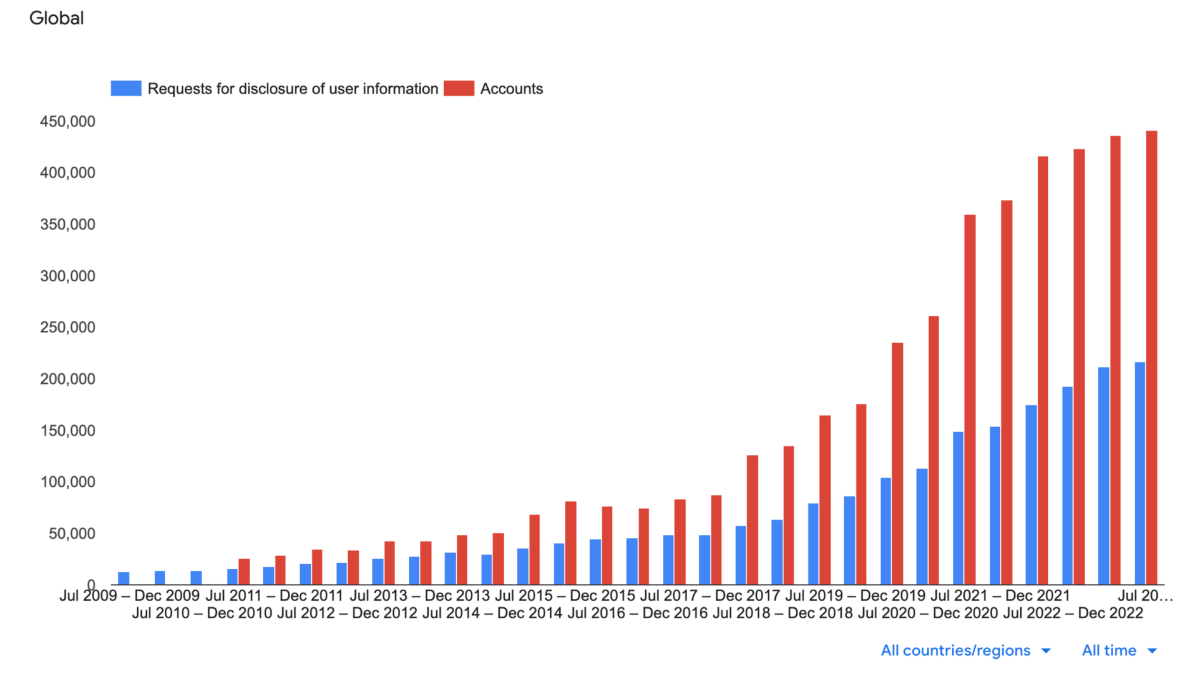
\includegraphics[scale=.4]{img/disclosure requests.png}
  \caption{Requests for user data disclosure during the years}
  \label{fig:disclosure-req}
\end{figure}
Another instrument that could be used to identify the suspect is the
\textbf{facial recognition}, that can be used only for terrorism
situations, but not in a systematic way.
\subsection{Detecting and Seizing Digital Evidence}
Anyone wanting to seize and validate digital/electronic evidences
(content of an e-mail or an entire hard-disk) has to respect two
fundamental \textbf{rules}: Bit-Stream Copy and Hash Function.
\subsubsection{Bit-Stream Copy}
\begin{boxH}
  A \textbf{bit-stream copy} can \textbf{clone} the \textbf{entire
  drive}.
\end{boxH}
It is a particular form of duplication in which the content of the
physical unit is read sequentially loading the minimum quantity of
data that can from time to time be directed, then recording it in the
same sequence on a standard binary file, generating a physical image
of the original medium.

\subsubsection{Hash Functions}
During the forensic analysis of modifiable media, the Hash 
guarantees the intangible nature of the data that it contains.
\begin{boxH}
  The Hash is a \textbf{one-way function}, by means of which a
  document of random length is converted into a limited and fixed
  length string.
\end{boxH}
This string represents a sort of ‘digital fingerprint’ of the non-
encrypted text, and is called the Hash Value or the Message Digest. If
the document is modified, even to the slightest extent, then the
fingerprint changes as well. In other words, by calculating and
recording the fingerprint, and then recalculating it, it can be shown
beyond all doubt whether the contents of the file, or the medium, have
been altered, even accidentally.\\

In any case we have two main problems while acquiring data: encryption
and jurisdiction. After all, the ISP, TELECO or even a bank does have
to cooperate and give out the data. Another big issue it the cloud
computing aspect, because the location of data is another big problem,
because it can be either:
\begin{itemize}
  \item \textbf{at rest}: does not reside on the device. 
  \item \textbf{in transit}: cannot be easily analysed because of
    encryption. 
  \item \textbf{in execution}: will be present only in the cloud
    instance
\end{itemize}
\textbf{Validation} of digital evidence is a very important step,
because it is the only way to prove that the evidence is authentic.
This is especially important for proof found on the internet. There
are some tools that can be used to validate digital evidence, such as
Web Forensics.\\
Another issue that has to be accouted for is the \textbf{chain of
custody}, that is the process of maintaining and documenting the
location and handling of evidence. After all, the bit is eternal, but
the storage medium is not.
\subsection{Validating Digital Evidence}
\subsection{Chain of Custody}
\subsection{Analysis of Digital Evidence}
\subsection{Presentation in Court}




\chapter{Cybercrime Convention}
\part{Technical part}
\chapter{Introduction to digital forensics}
First of all, we need to understand some basic concepts. \\
\textbf{Forensics analysis} is the process of investigating and
analyzing information to gather evidence to solve legal problems. In
order to do that, the collections, presevation and analysis or
presentation of digital evidence is required to support the
investigation. \textbf{Computer forensics} does just that.\\
Forensic science is not a new field, it has been around since the
ancient times. The first recorded use of forensic science was around
1900 BC in Babylon, where fingerprints were used to identify the 
author of a clay tablet. Digital forensics is a relatively new field,
it started in the 1980s with the advent of personal computers, for
example the first convicted person for digital crimes was Robert
Tappan Morris, who created the Morris Worm in 1988, and found out by
analyzing computer logs and network activity.
\begin{boxH}
  \textbf{Computer Forensics} is the \textbf{discipline} that combines elements
  of law and computer science to collect and analyze data from computer
  systems, networks, wireless communications, and storage devices in a way that
  is admissible as evidence in a court of law.
\end{boxH}
In general, when carrying out a forensic investigation, the following
questions are important to keep in mind to fully understand the 
crime scene:
\begin{itemize}
  \item \textbf{What} happened? What is the timeline of events?
  \item \textbf{Who} was involved?
  \item \textbf{When} did it happen?
  \item \textbf{Where} did it happen?
  \item \textbf{How} did it happen?
  \item \textbf{Why} did it happen?
  \item \textbf{How} did the incident occur?
\end{itemize}
All this questions allow to \textbf{support legal proceedings}, the mitigation
of damages and mature future prevention strategies.
\section{Computer forensics goals}
The main goals of computer forensics are:
\begin{enumerate}
  \item \textbf{retrieve} the \textbf{input} data(ie: what has been typed)
  \item \textbf{determine} the \textbf{actions} performed by the user (ie: what programs
    have been run)
  \item \textbf{analyze} the \textbf{used files} (ie: what files have been
    modified)
  \item \textbf{identify} the \textbf{damage} done to the system (ie: what
    files have been deleted)
\end{enumerate}
\begin{boxH}
  In essence, the goal of computer forensics is to \textbf{gain conprehansion}
  of \textbf{what happened}, at least technically speaking.
\end{boxH}

\section{CF terminology \& relevant concepts}
Before going any further, we need to understand some basic concepts
and terminology used in the field of computer forensics. 

For a definition of \textbf{digital evidence}, we can refer to
definition \ref{boxH:digital-evidence}. In general, we can expect to
deal with different types of digital evidence, because they can use
different level of \textbf{abstraction}. Most of the time that are
fragile, because they can be easily modified or destroyed, which is
undesirable during forensics investigations. Its also difficult to
correlate connection between data and real events, and to prove that
correlation in court. 

Another important concept is the \textbf{chain of custody}.
\begin{boxH}
  The \textbf{chain of custody} is the \textbf{documented} and
  \textbf{unbroken process} of handling evidence, from the moment it
  is collected to the moment it is presented in court.
\end{boxH}
This is important because it ensures that the evidence is not tampered
with, or even accessible by unauthorized personnel, and its most
important to ensure that the evidence is admissible in court. For
those reasons it requires knowledge about logging procedures, secure
storage and legal protocols, because many security measures are
required to ensure the integrity and confidentiality of the evidence.

\begin{boxH}
  \textbf{Data Acquisition} is the process of \textbf{collecting
  evidence} from devices without altering or damaging the original
  data.
\end{boxH}
This is one of the most subtle one, because it requires a deep
knowledge of how memory works, because it may be required to do disk
imaging when the data is at rest or even live data acquisition when
the data is in use. In any case, understanding of whats going on in
memory is required to avoid data corruption and tampering.

\begin{boxH}
  \textbf{Write Blockers} are hardware devices, or software tools,
  used to prevent any data from being written to a storage device
  during analysis, preserving the original data content.
\end{boxH}
Hardware write blockers are the most secure, because we don't have to
trust that the software is behaving correctly, but are also more 
expensive. In any case, they are fundamental for legally defensible
acquisitions.
\begin{boxH}
  \textbf{Forensic Image} is a \textbf{bit-by-bit copy} of digital
  media, including deleted files and data in slack space, which is an
  exact replica of the original device.
\end{boxH}
This is a strict requirement for digital forensics, because it allows
to preserve the original data, for example if the data is not exactly
copied the same way, the result of an hash function will be different.

\section{Forensics scenarios}
When doing a forensic investigation, there can be different scenarios
that can be encountered. Some common scenarios are:
\begin{itemize}
  \item internet abuse from employee
  \item computer-aided frauds
  \item data unauthorized manipulation, like data theft or disclosure
  \item computer/network damage assessment
  \item …and any time digital evidences may be involved in an incident
\end{itemize}
\section{Investigation phases}
The investigation process can be divided into several phases, at least
from a technical point of view. Those depends on the standards that
are followed in a given country where the investigation is taking 
place(fore example in America the NIST standards are followed).
\subsection{Identification}
Its the first step of the investigation, an it take place when the
crime scene has been accessed. The goal is to identify which are the
potential sources of relevant that, which will be used as digital
evidence if relevant.\\
Most of the time we have an overwhelming amount of data, but most of
it is not relevant to the investigation. Reducing the amount of data 
is also a goal of this phase. On the other hand, it is also possible
to miss some important data, so it is important to be careful.\\
It is important to recognize (all relevant) data sources before any
acquisition begins, like:
\begin{itemize}
  \item hard drives (HDD/SSD)
  \item memory (RAM)
  \item mobile devices (smartphones, tablets)
  \item cloud storage
  \item network traffic
  \item removable media (USB drives, DVDs)
  \item \dots 
\end{itemize}
The steps to follow in this phase are:
\begin{itemize}
  \item if possible, acquire data before reaching the crime
    scene(pre-analysis), instructing the staff to identify possible
    sources of evidence
  \item perform an \textbf{initial survey} of the scene (physical or
    network environment)
  \item \textbf{identify key devices} and data locations (local
    storage, remote servers, cloud services)
  \item \textbf{check} for \textbf{connected devices}, including
    peripherals like printers, removable media, or network-attached
    devices
  \item \textbf{map} all potential \textbf{data sources} using network
    topology
\end{itemize}
Pay much attention to the ephemeral storage of data, with reference to
the order of volatility. The order of volatility is a concept that
refers to the order in which data should be collected, based on how 
long it will be available.
\subsection{Collection}
After the identification phase, one must physically or remotely taking
possession of the evidence (e.g. a computer) and its connection (e.g.
Network or physical, like USB disk). The timing is most crucial in
this phase, while also maintaining the integrity of the evidence, to
minimize the risk of evidence tampering or data loss.\\
The steps to follow in this phase are:
\begin{itemize}
  \item isolate devices to prevent them from being tampered with
    remotely (e.g., disconnect them from the network)
  \item use devices to block external communication for mobile or
    wireless devices ( e.g. faraday bags)
  \item use network isolation tools for virtual and cloud environments
    to prevent remote access ( e.g security groups, virtual private
    cloud, firewall rule)
\end{itemize}
Its important to ensure the integrity of the evidence while
maintaining the system running, because shutting it down can cause the
loss of volatile data(e.g. RAM).
\subsection{Acquisition}
It refers to the process of electronically retrieving data by running various 
CF tools and software suite. Its a separate phase from the collection 
phase.

\begin{boxH}
  It's the process of creating a forensic copy (bit-by-bit image) of
  the original data to ensure that the acquired data is a faithful
  replica of the source while also maintaining data integrity
\end{boxH}
The acquisition method can be divided into two categories:
\begin{itemize}
  \item \textbf{Static acquisition}: the data is acquired while the
    system is turned off, and the data is at rest. 
  \item \textbf{Live acquisition}: the data is acquired while the
    system is running, and the data is in use. 
\end{itemize}
Depending on the method used, the acquisition can be done in different
ways and using different tools.

\subsubsection{Static acquisition}
Static acquisition can be carried out as follows:
\begin{itemize}
  \item shut them down carefully to avoid losing data ( e.g. for
    encrypted devices, consider methods for capturing data without
    triggering loss of access, for example before the decryption key is
    wiped from RAM)
  \item attach the device to a forensic workstation using a write blocker
  \item use forensic imaging tools to create a complete image of the
    storage device
  \item generate a hash value (e.g., SHA-256) of the original media
    before and after acquisition to verify integrity
  \item store the image on a secure forensic storage device
\end{itemize}
Be careful that the data is properly hashed and verified after the
acquisition.

\subsubsection{Live acquisition}
Live acquisition can be carried out as follows:
\begin{itemize}
  \item choose a method that minimizes system interference while
    capturing volatile data. This requires some knowledge of the
    system(FS, applications running, etc)
  \item dump RAM (memory acquisition) and capture data from running
    processes or network connections.
  \item perform network traffic capture
  \item document all acquisition actions and steps to ensure chain of
    custody and admissibility
  \item hash the volatile data wherever possible to maintain data
    integrity
\end{itemize}

\subsubsection{Integrity}
It ensure that the acquired data is an exact replica of the
original and has not been altered. To do so, some steps are required:
\begin{itemize}
  \item choose a method that minimizes system interference while
    generating a hash (MD5, SHA-256) of the acquired image or data dump
  \item compare the hash value to the original data hash (for static
    data) to verify its integrity
  \item document the hashing process, including the algorithms used and
    the results, in the chain of custody documentation
\end{itemize}

\begin{boxH}
  Any discrepancies in hash values would require re-acquisition and
  could damage the credibility of the evidence
\end{boxH}



\subsection{Evaluation}
Now that all the data has been collected, it is time to evaluate it.
In this phase the data is analyzed to substantiate claims and to
determine how they could be used against the suspect.
\subsection{Presentation}
At last, the evidence is presented in a clear and understandable way
to the court, in a manner which is suitable for lawyers, non-technical 
staff and the law.

\end{document}
